%!TEX root = /Users/dbreuer/Documents/Work/_FH/_Master/master_thesis/Main/Master Thesis.tex

\chapter{Prototypische Realisierung} % (fold)
\label{cha:prototypische_realisierung}

  Nachdem in das COSIMA-Projekt eingeführt und ein Szenario beschrieben wurde, dass zur Validierung der bisherigen Architektur dienen soll, wird in dem vorliegenden Kapitel die prototypische Realisierung der Architektur und des beschriebenen Szenario vorgestellt.
  
  In \citep{handbuch_der_software_architektur} wird beschrieben, dass bei der Entwicklung von Rahmenwerken in der Regel zuvor eine Reihe von ähnlichen Anwendungen entstehen, aus denen dann die Gemeinsamkeiten in ein Rahmenwerk extrahiert werden. Da es sich bei COSIMA zum Teil auch um ein Rahmenwerk handelt ($\to$ Abschnitt \ref{sub:framework_oder_architektur}) hätte bei der Entwicklung entsprechend verfahren werden können. Auf Grund der beschriebenen Neuartigkeit des Projekts wurde jedoch auf das in Kapitel \ref{cha:szenario} beschriebene szenariobasierte Vorgehen zurückgegriffen.
  
  Da bis zu diesem Zeitpunkt die Architektur nur konzeptionell existierte, boten sich bei der Realisierung und Validierung zwei Vorgehensweisen:

  \begin{enumerate}[\slshape a)]
    \item Die Implementierung einer prototypischen Anwendung für das in Abschnitt \ref{sub:das_anwendungsszenario} beschriebene Szenario, bei gleichzeitiger Umsetzung der Architektur \emph{oder}
    \item Die prototypische Realisierung der Architektur anhand eines von dem Szenario unabhängigen Anwendungsfall und anschließende Implementierung der eigentlichen Anwendung auf Basis dieser so entstandenen Architektur.
  \end{enumerate}
  
  Da die zu entwickelnde Anwendung und die zugrunde liegende Architektur beziehungsweise das verwendete Rahmenwerk relativ unabhängig voneinander sind, ist Alternative \emph{a)} nur bedingt empfehlenswert. Eine Dekorrelation beider Aspekte ist, wie bereits zuvor festgestellt notwendig und zudem gängige Praxis. Aus diesem Grund wurde sich für Alternative \emph{b)} entschieden. Demzufolge ist eine Implementierung\footnote{Die Implementierung sowohl der Architektur als auch des Szenario sind in der Programmiersprache Java ($\to$ \url{http://java.sun.com/j2se/1.5.0/}) in Version 5.0 durchgeführt worden.} in zwei, voneinander unabhängigen Stufen vorgenommen worden:
  
  \begin{enumerate}
    \item Prototypische Realisierung der wesentlichen Architekturmerkmale anhand eines einfachen Anwendungsfalls \emph{und}
    \item Implementierung des in \ref{sub:das_anwendungsszenario} beschriebenen Szenario auf Basis dieser Architektur.
  \end{enumerate}
  
  Im ersten Abschnitt dieses Kapitel wird daher zunächst detailliert auf die Umsetzung der Architektur eingegangen. Im Anschluss daran findet sich eine Erläuterung zur Implementierung des Szenario. Die Validierung und deren Ergebnisse werden dann im Anschluss in Kapitel \ref{cha:validierung_der_architektur} dargelegt.

\section{Realisierung der Architektur (Santiago)} % (fold)
\label{sec:realisierung_der_architektur}

  Bei dem gewählten \emph{bottom-up} Ansatz zur Entwicklung des Architekturprototypen musste zunächst ein geeigneter Anwendungsfall gefunden werden, der sich trotz einem Minimum an Komplexität dazu eignen musste, alle wesentlichen Architekturmerkmale extrahieren zu können. Zur besseren Kommunikation erhielt diese Anwendung den Codenamen \emph{Santiago} und ist formlos in Abbildung \ref{fig:images_Santiago_Anwendungsfall} strukturell dargestellt.

  \begin{figure}[!hb]
    \centering
      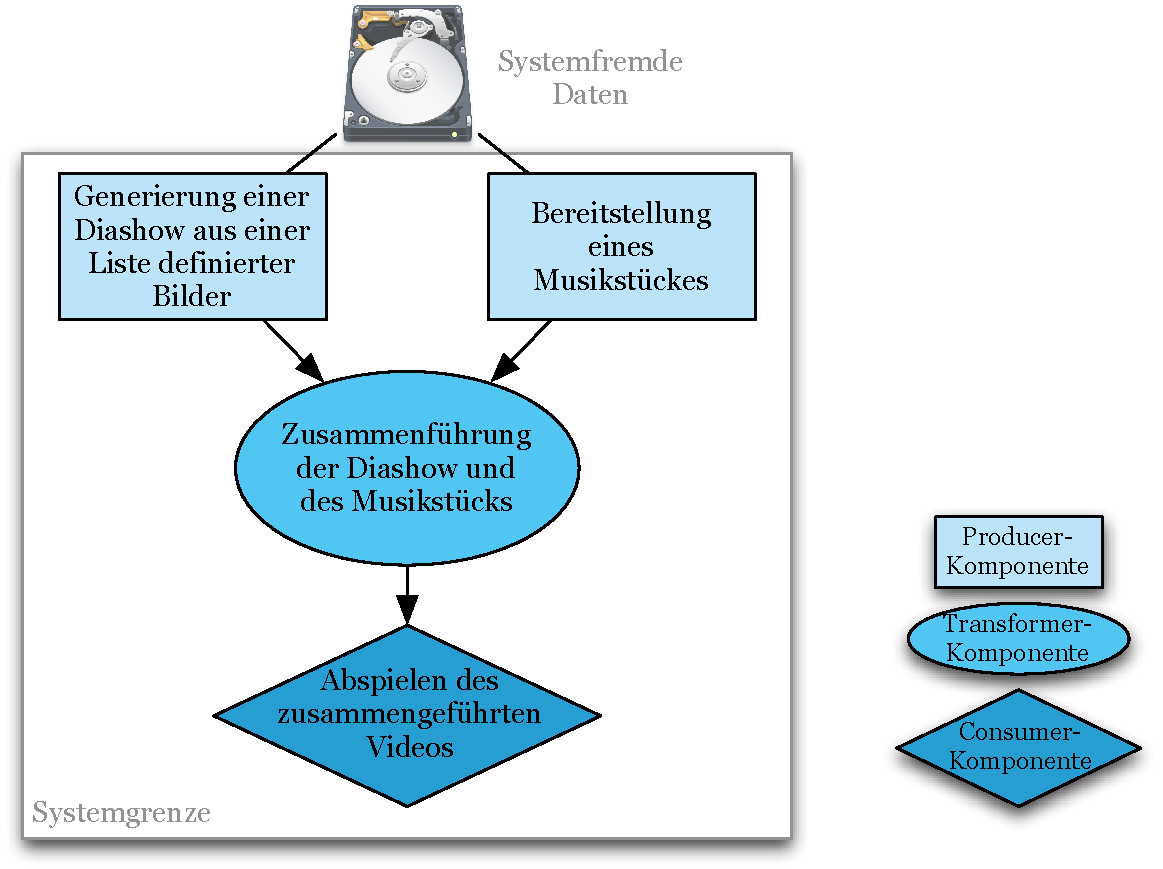
\includegraphics[width=.7\textwidth]{images/Santiago_Anwendungsfall.pdf}
    \caption{Anwendungsfall für die Realisierung der Architektur}
    \label{fig:images_Santiago_Anwendungsfall}
  \end{figure}

  \pagebreak

  Anhand lieser lassen sich leicht die drei wesentlichen Merkmale der Santiago Anwendung feststellen:
    
  \begin{itemize}
    \item Verarbeitung von unterschiedlichen Medien
    \item Umsetzung der einzelnen Verarbeitungsschritte in dedizierten Komponenten
    \item Anordnung dieser Komponenten nach dem Quelle-Komponente-Senke Prinzip
  \end{itemize}
  
  Trotz ihrer offensichtlichen Einfachheit konnte iterativ um diese Anwendung eine Architektur entwickelt werden, die alle notwendigen Charakteristika von COSIMA aufweist. Wie diese Entwicklung in den einzelnen Schritten im Detail aussah, beschreiben die folgenden Abschnitte.

\subsection{Erste Schritte} % (fold)
\label{sub:erste_schritte}

  In der ersten Iteration wurde lediglich ein einfaches Programm geschrieben, dass sequentiell jede der einzelnen Operationen auf den Medien ausführt und in Listing \ref{lst:santiago_plain} dargestellt ist. Die einzelnen Operationen wurden dabei bereits in dedizierten Klassen gekapselt und über statische Methoden zugänglich gemacht. Der Kontrollfluss ist in dieser Implementierung implizit über Objektaufrufe realisiert und durch die Ausführungsreihenfolge konkret festgelegt. Der Datenfluss entsteht durch die Übergabe beziehungsweise Rückgabe von Objektinstanzen.

\lstinputlisting[caption=\texttt{SantiagoPlain}-Klasse zur einfachen Ausführung des Anwendungsfalls,label=lst:santiago_plain,language=Java,firstline=11,morekeywords={[3]VideoPlayer,SlideshowGenerator,MusicOMat}]{../code/Santiago/src/main/java/de/fhkoeln/santiago/codesamples/SantiagoPlain.java}

  Die markierten Klassen implementieren dabei die jeweiligen Operationen in geeigneter Weise\footnote{Ein Einblick in die Implementierung der einzelnen Klassen ist an dieser Stelle nicht weiter relevant. Der vollständige Quellcode findet sich auf der Begleit-CD zu dieser Arbeit.}. Den Zugriff auf diese Operationen über Klassenmethoden zu realisieren eignet sich jedoch nicht für den Einsatz in verteilten Umgebungen: Eine parallele Verwendung ein und der selben Komponente wäre so nur schwer umsetzbar. In der nächsten Iteration war es daher notwendig, die Ausführung der Operationen auf Objektebene zu implementieren. Gleichzeitig sollte der entsprechende Aufruf dabei polymorphisch erfolgen können. Die Umsetzung dieser beiden Anforderungen erfolgte über die Etablierung der abstrakten Oberklasse \verb!AbstractComponent! (siehe Listing \ref{lst:abstract_component_simple_class}), da alle Komponenten zwei wesentliche Gemeinsamkeiten aufweisen, \emph{a)} sie Übergabe von Eingabeparametern und \emph{b)} die Ausführung der Operation unter Berücksichtigung dieser Parameter. Die Oberklasse definiert dabei drei Methoden: Die Methode \verb!setInput(String [] inputs)!, um die notwendigen Parameter zu setzen; Die Methode \verb!execute()! als nach außen sichtbare Schnittstelle, um die Operation zu starten und die Methode \verb!_execute()! in der die eigentliche Operation intern implementiert ist.
  
  \lstinputlisting[caption=Einfache \texttt{AbstractComponent}-Klasse,label=lst:abstract_component_simple_class,language=Java,firstline=8,morekeywords={[3]execute,getInput,setInput}]{../code/COSIMA/src/main/java/de/fhkoeln/cosima/codesamples/AbstractComponent.java}
  
  Das ausführende Programm aus Listing \ref{lst:santiago_plain} kann nun die generalisierten Komponenten mit ihren homogenen Schnittstellen verwenden um die einzelnen Operationen anzustoßen. Die entsprechenden Änderungen der Anwendung sind dabei in Listing \ref{lst:santiago_plain_with_general_components} dargestellt. Als eine erste Abstraktion der Parameter dient in diesem Fall noch ein primitives String-Array, im weiteren Verlauf wird daraus ein vollständiges \emph{Value-Object} \citep[S. 486]{fowler03peaa} entstehen. Die Implementierung der \verb!execute()!-Methode ist nach dem \emph{Template Method} Entwurfsmuster vorgenommen worden \citep[325]{design_patterns}\footnote{In späteren Iterationen lassen sich so leicht Funktionalitäten hinzufügen, die vor oder nach der eigentlichen Operation durchgeführt werden müssen.}.

  \lstinputlisting[caption=Erweitertes Santiago Programm mit generalisierten Komponenten,label=lst:santiago_plain_with_general_components,language=Java,firstline=23,lastline=36,morekeywords={[3]AbstractComponent}]{../code/Santiago/src/main/java/de/fhkoeln/santiago/codesamples/SantiagoPlainWithGeneralComponents.java}
  
  Für die nächste Iteration war es notwendig, wie bereits in Abbildung \ref{fig:schema_des_anwendungsszenario} dargestellt, dass eine Producer-Komponente das Musikstück erst innerhalb der Systemgrenzen \emph{bekannt machen} muss. Der Grund dafür ist, dass innerhalb einer COSIMA-Anwendung eine Transformer-Komponente nur Mediendaten verarbeiten kann, die bereits im System vorhanden sind, also über den Medienbroker abgerufen werden können. Im Kontext von COSIMA hat das die Bedeutung, dass ein Medienobjekt erzeugt und über den Medienbroker bereitgestellt wird. Für die Santiago Anwendung bedeutet es momentan lediglich, dass das String-Objekt \verb!musicPath! durch eine Instanz der \verb!MusicProvider!-Klasse (siehe Listing \ref{lst:santiago_plain_with_music_provider}) dem String-Objekt \verb!music! zugewiesen wird.
  
  \lstinputlisting[caption=Integration einer dedizierter Komponente zur Bereitstellung der Musik,label=lst:santiago_plain_with_music_provider,language=Java,firstline=23,lastline=26,morekeywords={[3]MusicProvider}]{../code/Santiago/src/main/java/de/fhkoeln/santiago/codesamples/SantiagoPlainWithMusicProvider.java}
  
  Dabei ist natürlich zu beachten, dass der \verb!MusicOMat!-Instanz nicht länger die Referenz auf das \verb!musicPath!-Objekt, sondern auf das \verb!music!-Objekt übergeben wird.
  
  Nachdem die notwendigen Komponenten zur Medienverarbeitung implementiert wurden, musste in der nächsten Iteration der Kontrollfluss über eine deklarative Beschreibung anzugeben sein. Des Weiteren musste diese Beschreibung durch eine dedizierte Komponente interpretiert und ausgeführt werden. Die Entwicklung dieser Ablaufbeschreibung und ihrer ausführenden Instanz wird im folgenden Abschnitt näher beschrieben.
  
% subsection erste_schritte (end)
  
\subsection{Einführung einer deklarativen Ablaufbeschreibung} % (fold)
\label{sub:einfuehrung_einer_deklarativen_ablaufbeschreibung}

  Nachdem die einzelnen Komponenten über eine einheitliche Schnittstelle ausführbar gemacht worden sind, war der nächste Schritt, eine Komposition der einzelnen Komponenten zu realisieren. Im Rahmen der prototypischen Implementierung wurde sich für eine Orchestrierung ($\to$ Abschnitt \ref{def:orchestrierung}) entschieden, wodurch eine zentral ausführende Einheit umgesetzt werden musste, die eine deklarative Ablaufbeschreibung interpretiert und ausführt. Um im Rahmen der prototypischen Umsetzung ein möglichst gutes Verständnis dieser Komponente entwickeln zu können, wurde bewusst darauf verzichtet, bestehende Lösungen wie etwa BPEL einzusetzen. Ein weiterer Grund dafür ist, dass nicht geklärt ist inwieweit sich BPEL überhaupt für den Einsatz in einem Multimediakontext eignet, wie auch schon bei \citep{samma08} ausgeführt. Dort wird der Einsatz von BPEL für Multimediaanwendungen erst nach einer entsprechenden Erweiterung empfohlen.
  
  Daher wurde eine einfache properitäre Kompositionseinheit selbst implementiert. Auf Grund der so entstandenen Minimierung von Abhängigkeiten komplexer Bibliotheken Dritter, konnte auch die Gesamtkomplexität minimal gehalten und dadurch dem Ziel die Architektur an sich zu validieren mehr Rechnung getragen werden.
  
  \begin{kasten}
    \minisec{Der Begriff "`Workflow"'} % (fold)
    \label{msec:der_begriff_workflow}

      Bevor sich der Implementierung der Servicekomposition zugewandt wird, soll noch eine Abgrenzung der Begriffe \emph{Workflow} und \emph{Prozess} erfolgen. Im Rahmen der Implementierung ist die Verwendung dieser beiden Begriffe nicht im Kontext von Geschäftsprozessen zu verstehen, wie sie bei \citep{samma08} ebenfalls im gegebenen Zusammenhang mit dem COSIMA-Projekt behandelt werden. Im Kontext dieser Arbeit hat daher die folgende Definition von Workflow Gültigkeit:
      
      \begin{definition}[Workflow]\label{def:workflow}
        "`The computerised facilitation or automation of a process, in whole or part."' \emph{\citep[S. 54]{hollingsworth1995wmc}}
      \end{definition}
      
      Wesentlich dabei ist die computergestützte Automatisierung eines Prozesses, es fehlen demnach also manuelle Aktivitäten. Ein Prozess ist in diesem Kontext wie folgt definiert:
      
      \begin{definition}[Prozess]\label{def:prozess}
        "`A co-ordinated (parallel and/or serial) set of process activity(s) that are connected in order to achieve a common goal. Such activities may consist of manual activity(s) and/or workflow activity(s)."' \emph{\citep[S. 52]{hollingsworth1995wmc}}
      \end{definition}
      
      Der Prozess beinhaltet demnach eine Reihe von definierten Aktivitäten, die der Erreichung eines bestimmten Ziels dienen. Diese Aktivitäten können dabei entweder manueller oder automatisierter Natur sein. Die Definition der Aktivitäten geschieht dabei in Form einer \emph{Prozessdefinition}. Da innerhalb der Santiago-Anwendung als auch in dem Anwendungsszenario aus Abschnitt \ref{sub:das_anwendungsszenario} keine manuellen Aktivitäten enthalten sind, kann im weiteren Verlauf daher ausschließlich von Workflow gesprochen werden. Demnach ist auch nur der Teil der Prozessdefinition relevant, der die automatisierten Aspekte des Prozesses beinhaltet. Diesen Teil bezeichnet man als \emph{Workflowdefinition} \citep[S. 52]{hollingsworth1995wmc}.
      
      Diese sehr vereinfachte Begriffliche Verwendung ist für eine weitere Bearbeitung im Rahmen des COSIMA-Projekts in jedem Fall zu erweitern. Die Erweiterungen müssen sich dabei auch in der Implementierung der Architektur wieder finden lassen. Als Ausgangspunkt für die weiteren Betrachtungen sollte die Arbeit von \citep{samma08} herangezogen werden.
      
    % minisec einschub_der_begriff_workflow (end)
  \end{kasten}

  Die Implementierung der Servicekomposition innerhalb der Santiago-Anwendung besteht im wesentlichen aus vier Komponenten:
  
  \begin{enumerate}
    \item Eine Schnittstelle, die die Ablaufbeschreibung in der Anwendung darstellt;
    \item Eine deklarative Ablaufbeschreibung in einem gegebenen Format;
    \item Eine Klasse, die die einzelnen Elemente in dieser Beschreibung repräsentiert;
    \item Eine ausführende Komponente.
  \end{enumerate}
  
  Das \verb!WorkflowDefinition!-Interface stellt die Schnittstelle für die Abbildung und den Zugriff auf die Ablaufbeschreibung dar und ist in Listing \ref{lst:workflow_definition_interface} zu sehen\footnote{Eine Erläuterung des Begriffs "`Workflow"' findet sich in dem gleichnamigen Kasten.}.

\lstinputlisting[caption=Das \texttt{WorkflowDefinition}-Interface,label=lst:workflow_definition_interface,language=Java,firstline=12]{../code/COSIMA/src/main/java/de/fhkoeln/cosima/workflow/WorkflowDefinition.java}

  Diese einfache Schnittstelle bietet dem Client zum einen an, über die \verb!size()!-Methode die Größe aller auszuführenden Elemente nachzufragen und über die Implementierung des \emph{Iterator}-Pattern \citep[S. 257]{design_patterns} alle Elemente in ihrer jeweils definierten Sequenz. Die entsprechende Realisierung des \verb!WorkflowDefinitionIterator! ist in Listing \ref{lst:workflow_definition_iterator} zu sehen. Die \verb!next()!-Methode liefert dabei immer ein \verb!java.util.Set! von \verb!WorkflowElement!-Objekten zurück, die als nächstes ausgeführt werden müssen, allerdings ohne die Notwendigkeit sie in einer definierten Reihenfolge auszuführen\footnote{Für die erfolgreiche Ausführung der Santiago-Anwendung ist es irrelevant, ob zuerst die Diashow erstellt wird und dann das Musikstück bereitgestellt wird oder vice versa.}.

\lstinputlisting[caption=Implementierung der \texttt{WorkflowDefinitionIterator}-Klasse,label=lst:workflow_definition_iterator,language=Java,linerange={12-13,31-92}]{../code/COSIMA/src/main/java/de/fhkoeln/cosima/workflow/WorkflowDefinitionIterator.java}

  Die Ablaufbeschreibung selbst wurde für Santiago im YAML\abk{YAML}{YAML Ain't Markup Language}-Format angebeben\footnote{YAML ist eine datenzentierter Serialisierungsstandard für alle Programmiersprachen, der sehr menschenlesbar ist (siehe \url{http://www.yaml.org}).}. Es wurde sich bewusst für ein datenzentiertes Format und nicht für ein dokumentenzentriertes Format wie XML\abk{XML}{eXtensible Markup Language} entschieden, um die bereits erwähnte Abgrenzung zu BPEL und Geschäftsprozessen\footnote{Bei der Beschreibung von Geschäftsprozessen lässt sich sehr viel eher von einem Dokument sprechen, dass entsprechend in einem System modelliert werden sollte.} auch in der Implementierung herauszustellen. Die Ablaufbeschreibung, die den Anwendungsfall in Santiago darstellt ist in Listing \ref{lst:abstract_workflow_definition_in_yaml} zu sehen.

\lstinputlisting[caption=Einfache deklarative Ablaufbeschreibung für Santiago im YAML-Format,label=lst:abstract_workflow_definition_in_yaml,language=YAML]{../code/Santiago/src/main/resources/workflow_definition.yml}

  Wie im Listing zu sehen ist, besteht die Ablaufbeschreibung aus vier Teilbereichen, die jeweils durch die Zeichenkette \verb!---! getrennt sind. Jeder Bereich steht dabei für ein Element, dass später im Workflow ausgeführt werden muss und beschreibt dementsprechend eine der vier medienverarbeitenden Komponenten innerhalb der Anwendung. Innerhalb jedem dieser Elemente sind die zur Ausführung des Workflows notwendigen Attribute einer Komponente definiert. Ein Attribut wird dabei durch ein \verb!key: value!-Paar markiert, wobei der Doppelpunkt (\verb!:!) den \verb!key! von dem \verb!value! trennt. Attribute können dabei verschachtelt werden, was durch eine Einrückung dargestellt wird\footnote{Eine genaue Spezifikation zu der aktuellen YAML Version 1.2 findet sich unter \url{http://yaml.org/spec/1.2}.}. Im Folgenden sind die wesentliche Attribute eines Elements zusammengefasst:
  
  \begin{description}
    \item[Beschreibung (\texttt{description})] Eine informelle Beschreibung der jeweiligen Komponente.
    \item[URI (\texttt{uri})] Die URI anhand derer später die entsprechende Komponente lokalisiert und ausgeführt werden kann.
    \item[Eingänge (\texttt{input})] Eine Liste von Eingabedaten. Eingabedaten können entweder \emph{extern} (in diesem Beispiel also die Musikdatei und die Bilder der Diashow) oder \emph{intern} sein (die Diashow und die Diashow mit Musik). Die einzelnen Eingaben wird über eine URI referenziert.
    \item[Ausgänge (\texttt{output})] Eine Liste von Ausgabedaten. Eine hier formulierte Ausgabe ist zur Zeit immer systemintern. Auch die Ausgaben werden über eine URI referenziert\footnote{Zu beachten ist, dass es sich bei diesen Referenzen nicht zwangsläufig um Referenzen auf die eigentlichen Medien handeln muss: Sie werden zur Verknüpfung der Ein- und Ausgänge der einzelnen Komponenten während der Ausführung des Workflows verwendet.}.
    \item[Vorgänger (\texttt{predecessors})] Eine Liste von Komponenten, die \emph{vor} dieser Komponente ausgeführt werden müssen. Die Komponenten werden dazu durch ihre URI referenziert. Elemente ohne Vorgänger werden als erstes ausgeführt.
    \item[Nachfolger (\texttt{successors})] Eine Liste von Komponenten, die \emph{nach} dieser Komponente ausgeführt werden müssen. Die Komponenten werden dazu durch ihre URI referenziert. Elemente ohne Nachfolger markieren das Ende des Workflows.
  \end{description}

  Neben der eigentlichen Ablaufbeschreibung im YAML-Format ist darüber hinaus noch eine Klasse notwendig, die das \verb!WorkflowDefinition!-Interface implementiert und die in der Lage ist, die angegebene Ablaufbeschreibung einzulesen. Die einzelnen Elemente der abstrakten Ablaufbeschreibung werden auf Programmebene dabei durch Instanzen der Klasse \verb!WorkflowElement! repräsentiert. Die Klasse implementiert dabei die die einzelnen \verb!key: value!-Paar entsprechend als Attribute, die über \emph{Getter}-Methoden nach außen verfügbar gemacht werden. Die \verb!YamlWorkflowDefinition!-Klasse setzt dafür auf jeder Instanz eines \verb!WorkflowElement! die entsprechenden Werte über die gleichnamigen \emph{Setter}-Methoden automatisch. Die \verb!YamlWorkflowDefinition!-Implementierung findet sich in Listing \ref{lst:yaml_workflow_definition} und das vollständige Listing \ref{lst:workflow_element} zu der \verb!WorkflowElement!-Klasse findet sich im Anhang.

  \lstinputlisting[caption=Implementierung des \texttt{WorkflowDefinition}-Interface auf YAML-Basis,label=lst:yaml_workflow_definition,language=Java,linerange={12-13,35-76}]{../code/COSIMA/src/main/java/de/fhkoeln/cosima/workflow/YamlWorkflowDefinition.java}

  Die \verb!WorkflowDefinition! ist jedoch lediglich die programmatische Repräsentation der deklarativen Beschreibung, um diese auszuführen bedarf es einer weiteren Komponente, der \emph{Workflow Engine} \citep[S. 53]{hollingsworth1995wmc}. Sie wird in COSIMA durch die abstrakte \verb!WorkflowEngine!-Klasse realisiert ($\to$ Listing \ref{lst:workflow_engine}). Die jeweiligen Unterklassen müssen dabei entsprechend die \verb!execute()!-Methode überschreiben.
  
  \lstinputlisting[caption=Abstrakte \texttt{WorkflowEngine}-Klasse,label=lst:workflow_engine,language=Java,linerange={12-13,16-38}]{../code/COSIMA/src/main/java/de/fhkoeln/cosima/workflow/WorkflowEngine.java}
  
  Eine erste einfache Implementierung der abstrakten \verb!WorkflowEngine!-Klasse ist in Listing \ref{lst:simple_workflow_engine} dargestellt.

  \lstinputlisting[caption=Implementierung einer einfachen Workflow Engine,label=lst:simple_workflow_engine,language=Java,linerange={12-13,23-60},morekeywords={[3]WorkflowDefinition,workflowStore,WorkflowElement}]{../code/COSIMA/src/main/java/de/fhkoeln/cosima/workflow/SimpleWorkflowEngine.java}

  Die Instanziierung der einzelnen Komponenten innerhalb der \verb!SimpleWorkflowEngine! geschieht dabei unter zur Hilfenahme der Java Reflection API\abk{API}{Application Programming Interface} (Zeile 54 und 55 in Listing \ref{lst:simple_workflow_engine}). Dies gelingt, da in der Ablaufbeschreibung als URI jeder Komponente der vollständig klassifizierende Java-Klassenname angegeben ist. Für den Einsatz in einer verteilten Umgebung ist diese Implementierung jedoch völlig ungeeignet. Später werden die einzelnen Komponenten daher als \emph{Web Services} implementiert werden ($\to$ Abschnitt \ref{sub:extraktion_der_komponenten_als_dienste}). Ein weiterer Punkt von Interesse in dieser Implementierung ist die Notwendigkeit den aktuellen Fortschritt der Ausführung nachzuhalten. Dies wird über die Einführung des lokalen \verb!workflowStore!-Objekts erreicht. Für die Umsetzung komplexerer Abläufe scheint es jedoch sinnvoll zu sein, dass der ausführenden Komponente ein Zustandsautomat zu Grunde gelegt wird, wie es bei \citep{biornstad2006cfs} propagiert und unter anderem auch von BPEL umgesetzt wird.
  
  Das Santiago Programm aus den bisherigen Listings lässt sich durch die in diesem Abschnitt eingeführten Erweiterungen allein auf die Instanziierung einer \verb!WorkflowDefinition! und die Ausführung der \verb!SimpleWorkflowEngine! mit dieser Definition reduzieren (Listing \ref{lst:santiago_plain_with_workflow_definition}).
  
  \lstinputlisting[caption=Santiago Programm mit deklarativer Ablaufbeschreibung,label=lst:santiago_plain_with_workflow_definition,language=Java,firstline=19,lastline=34,morekeywords={[3]WorkflowDefinition,SimpleWorkflowEngine}]{../code/Santiago/src/main/java/de/fhkoeln/santiago/codesamples/SantiagoPlainWithWorkflowDefinition.java}
  
  Nachdem eine deklarative Ablaufbeschreibung eingeführt wurde und die grundsätzliche Möglichkeit geboten ist, diese Beschreibung auszuführen, ist der nächste Schritt die Umsetzung der Medienobjekte-Modellierung. Diese wird im nächsten Abschnitt behandelt.
  
% subsection einfuewhrung_einer_deklarativen_ablaufbeschreibung (end)

\subsection{Explizite Umsetzung des Datenfluss und Einführung des Medienobjekts} % (fold)
\label{sub:explizite_umsetzung_des_datenfluss}

  In Abschnitt \ref{ssub:medienobjekt} wurde bereits darauf hingewiesen, dass zwischen Kontrollfluss und Datenfluss innerhalb einer SOA unterschieden werden muss. Im vorherigen Abschnitt wurden entsprechend die Komponenten realisiert, die dem Kontrollfluss zuzuordnen sind. In diesem Abschnitt werden die Komponenten implementiert, die zur Umsetzung des Datenfluss notwendig sind.
  
  Im ersten Schritt soll zunächst ein \emph{Value-Object} eingeführt werden, wie in Abschnitt \ref{sub:erste_schritte} bereits angekündigt. Dieses soll dazu dienen die notwendigen Ein- und Ausgabewerte einzelner \verb!AbstractComponent!-Instanzen zu kapseln und leichter übertragbar zu machen. Die Implementierung dieses Objekt in Form der IODescriptor-Klasse ist in Listing \ref{lst:io_descriptor} dargestellt\footnote{Die Implementierung der \lstinline[basicstyle=\ttfamily\footnotesize]!equals()! und \lstinline[basicstyle=\ttfamily\footnotesize]!hash()!-Methoden sind zur Erfüllung des Value-Object-Pattern notwending \citep[S. 486]{fowler03peaa}.}.

  \lstinputlisting[caption=\texttt{IODescriptor} als Implementierung des \emph{Value-Object} Pattern,label=lst:io_descriptor,language=Java,linerange={12-13,26-79,85-88,102-103}]{../code/COSIMA/src/main/java/de/fhkoeln/cosima/services/IODescriptor.java}
  
  Diese Änderungen haben dabei keinerlei Auswirkungen auf das Santiago Programm selbst. Dieses stellt sich immer noch genauso dar wie in Listing \ref{lst:santiago_plain_with_workflow_definition}. Änderungen müssen nur, wie in Listing \ref{lst:simple_workflow_engine_with_io_descriptor} dargestellt, an der \verb!SimpleWorkflowEngine!-Klasse vorgenommen werden. Die Anpassungen an der \verb!AbstractComponent!-Klasse, dass die Methoden \verb!execute()! und \verb!setInput()! je eine \verb!IODescriptor!-Instanz zurückgeben beziehungsweise entgegennehmen, werden an dieser Stelle ausgespart.
  
  \lstinputlisting[caption=Erweiterung der einfachen Workflow-Engine um den \texttt{IODescriptor},label=lst:simple_workflow_engine_with_io_descriptor,language=Java,firstline=28,lastline=57,morekeywords={[3]IODescriptor}]{../code/COSIMA/src/main/java/de/fhkoeln/cosima/workflow/SimpleWorkflowEngineWithIO.java}
  
  Wesentlich entscheidender für die Realisierung des Datenfluss ist jedoch die Implementierung des Medienobjekts, wie es in \ref{ssub:medienobjekt} konzeptioniert wurde. Diese Erweiterung hat dabei nur Auswirkungen auf die \verb!AbstractComponent!-Klasse und ihre Unterklassen, nicht jedoch auf die jeweiligen \verb!WorkflowEngine!-Implementierungen.
  
  Das Medienobjekt selbst ist wie bereits ausgeführt und in Abbildung \ref{fig:medienobjekt} zu erkennen, nach dem \emph{Composite}-Pattern implementiert. Bei der Umsetzung des Composite-Pattern sind in der Regel\footnote{Alternativ ließe sich die polymorphische Verwendung von \lstinline[basicstyle=\ttfamily\footnotesize]!Composite! und \lstinline[basicstyle=\ttfamily\footnotesize]!Leaf!-Objekten über die Einführung eines \lstinline[basicstyle=\ttfamily\footnotesize]!Component!-Interface erreichen.} drei Klassen zu implementieren:
  
  \begin{description}
    \item[Component]   Die Klasse von der die anderen beiden jeweils vererben (hier die \verb!MediaComponent!-Klasse). In dieser Klasse werden auch die Methoden zum traversieren der Composite-Objekte definiert.
    \item[Composite]   Die Klasse, in der mehrere Component-Objekte zusammengefasst werden (hier die \verb!MediaContainer!-Klasse).
    \item[Leaf]   Die Klasse, die einen Endpunkt in der Hierarchie repräsentiert (hier die \verb!Media!-Klasse).
  \end{description}
  
  Zur Realisierung der Santiago-Anwendung ist die Verwendung von \verb!MediaContainer!-Instanzen nicht notwendig, daher wird darauf auch nicht weiter eingegangen. Die Implementierungen der anderen beiden Klassen sind in Listing \ref{lst:abstract_media} und \ref{lst:media_data} zu sehen.

  \lstinputlisting[caption=\texttt{MediaComponent}-Klasse als \emph{Component} im Composite-Pattern,label=lst:abstract_media,language=Java,linerange={12-13,31-149,157-158}]{../code/COSIMA/src/main/java/de/fhkoeln/cosima/media/MediaComponent.java}

  \lstinputlisting[caption=\texttt{Media}-Klasse als \emph{Leaf} im Composite-Pattern,label=lst:media_data,language=Java,linerange={12-13,23-46,60-61}]{../code/COSIMA/src/main/java/de/fhkoeln/cosima/media/Media.java}
  
  Jedes Medienobjekt, unabhängig davon ob es \emph{Leaf} oder \emph{Composite} ist, verfügt über einen Namen und einen Namensraum. Aus diesen beiden Angaben lässt sich die URI über die \verb!getUri()!-Methode ermitteln. Später lässt sich mit dieser URI ein Medienobjekt eindeutig im Kontext eines Medienbroker lokalisieren.
  
  Zur Speicherung der Medienobjekte über den Medienbroker implementiert die \verb!Media-Component!-Klasse das \verb!java.lang.Serializable!-Interface. Zusätzlich muss jede Unterklasse das Feld \verb!serialVersionUID! definieren.
  
  Zur Persistierung der eigentlichen Mediendaten sowie um Medienobjekte vergleichbar zu machen wurden zusätzlich die Methoden \verb!equals()! und \verb!hash()! überschrieben.
  
  Des Weiteren hat jedes Medienobjekt eine Reihe von Metadaten assoziiert. Jede Metadata muss dabei das \verb!Metadata!-Interface implementieren. Es definiert dabei lediglich die Funktionalität, dass einem Schlüssel in einem definierten Namensraum ein beliebiger Wert zugewiesen wird (siehe Listing \ref{lst:metadata_interface}). Zusätzlich verfügt jedes \verb!Metadata!-Objekt über eine URI zur eindeutigen Identifikation. Zu diesem Zeitpunkt existiert jedoch noch keine Implementierung dieser Schnittstelle, denkbar wäre aber zum Beispiel eine Implementierung auf Basis des Dublin Core Metadaten Standards\footnote{Die \emph{Dublin Core Metadata Initiative} ist eine offene Organisation mit dem Ziel einen flexiblen und austauschbaren online Standard für Metadaten zu schaffen, der die unterschiedlichsten Anwendungen erlaubt (\url{http://dublincore.org/}).}.
  
  \lstinputlisting[caption=\texttt{Metadata}-Interface als abstrakte Repräsentation von Metadaten,label=lst:metadata_interface,language=Java]{../code/COSIMA/src/main/java/de/fhkoeln/cosima/media/Metadata.java}
  
  Medienobjekte sind weder "`abspielbar"' noch lassen sich auf ihnen medienverarbeitende Operationen durchführen, sie sind wie schon in Abschnitt \ref{ssub:medienobjekt} erwähnt, lediglich reichhaltige Referenzen auf die eigentlichen Daten. Der Zugriff auf eben diese Daten erfolgt über die \verb!getPlayableData()!-Methode. Die Methode ist nach dem \emph{Lazy-Load}-Pattern \citep[S. 200]{fowler03peaa} implementiert, so dass die potentiell sehr großen Mediendaten erst geladen werden, wenn sie tatsächlich benötigt werden. Wie das Laden uns Speichern von Medienobjekten an sich implementiert ist, stellt der nachfolgende Abschnitt im Detail vor.
 
\subsubsection{Speichern und Laden von Medienobjekten} % (fold)
\label{ssub:speichern_und_laden_von_medienobjekten}

  Bei dem Umgang mit Medienobjekten müssen zwei unterschiedliche Aspekte betrachtet werden:
  
  \begin{itemize}
    \item Die Vermittlung der Medienobjekte
    \item Die Persistierung der Mediendaten
  \end{itemize}
  
  Die Trennung ist bereits auf Modellebene vorgesehen worden, wie in Abbildung \ref{fig:medienobjekt} dargestellt ist. Diese Trennung soll daher entsprechend auch im Code umgesetzt werden.
  
  Die Vermittlung der Medienobjekte übernimmt ein Medienbroker. Der wesentliche Teil der zugehörigen Schnittstelle ist in Listing \ref{lst:media_broker} zu sehen. Im Rahmen dieser Arbeit wird die \verb!MemcachedMediaBroker!-Implementierung des \verb!MediaBroker!-Interface verwendet. Die Speicherung der einzelnen Medienobjekte wird dabei über eine Objektserialisierung und deren Hinterlegung in einem \texttt{\slshape{memcached}}\emph{-Server}\footnote{\lstinline[basicstyle=\ttfamily\footnotesize]!memcached! ist ein ACID\abk{ACID}{Atomicity, Consistency, Isolation, Durability}-konformer, hochperformanter verteilter Objektspeicher (siehe \url{http://www.danga.com/memcached/})} realisiert. Der \verb!memcached!-Server erlaubt die leichte Vermittlung und Speicherung von Medienobjekten in einem verteilten System und war daher optimal für den Einsatz in einem Prototypen geeignet.
  
  \lstinputlisting[caption=Das \texttt{MediaBroker}-Interface zur Vermittlung von Medienobjekten,label=lst:media_broker,language=Java,linerange={12-13,27-40,60-61}]{../code/COSIMA/src/main/java/de/fhkoeln/cosima/media/mediabroker/MediaBroker.java}

  Die Persistierung der eigentlichen Daten übernimmt die \verb!MediaStore!-Komponente, deren Schnittstelle in Listing \ref{lst:media_store_interface} zu sehen ist. Die Implementierung innerhalb dieser Arbeit speichert die Mediendaten auf dem Dateisystem\footnote{Für den Einsatz in einer verteilten Umgebung lässt sich einfach ein NFS\abk{NFS}{Network File System}-Mount verwenden.}. Für eine weitere Entwicklung würde sich hier die Integration eines verteilten Dateisystems oder des bereits erwähnten MultiMonster-Medienservers anbieten.

  \lstinputlisting[caption=Das \texttt{MediaStore}-Interface zur Persistierung von Medien,label=lst:media_store_interface,language=Java,linerange={12-13,26-47}]{../code/COSIMA/src/main/java/de/fhkoeln/cosima/media/mediabroker/storage/MediaStore.java}

  Die wesentlichen Methoden des \verb!MediaBroker!-Interface sind die Methoden \verb!store()! und \verb!retrieve()!. Die \verb!store()!-Methode nimmt dabei ein Medienobjekt entgegen, legt es in der Speicherlösung der jeweiligen \verb!MediaBroker!-Implementierung ab und reicht das Medienobjekt an die assoziierte \verb!MediaStore!-Instanz weiter. Am Ende wird die Referenz im übergebenen Medienobjekt auf \verb!null! gesetzt, damit im Anschluss diese Referenz nicht länger genutzt werden kann. Die Realisierung dieser Methode in der \verb!MemcachedMediaBroker!-Implementierung ist in Listing \ref{lst:store_method_in_memcached_media_broker} zu sehen.

  \lstinputlisting[caption=Implementierung der \texttt{store()}-Methode im  \texttt{MemcachedMediaBroker},label=lst:store_method_in_memcached_media_broker,language=Java,firstline=74,lastline=87]{../code/COSIMA/src/main/java/de/fhkoeln/cosima/media/mediabroker/MemcachedMediaBroker.java}
  
  Zur besseren Veranschaulichung, wie die Speicherung von Medienobjekt abläuft, dient das in Abbildung \ref{fig:speichern_von_medienobjekten} dargestellte Sequenzdiagramm.

  \begin{figure}[!ht]
    \centering
      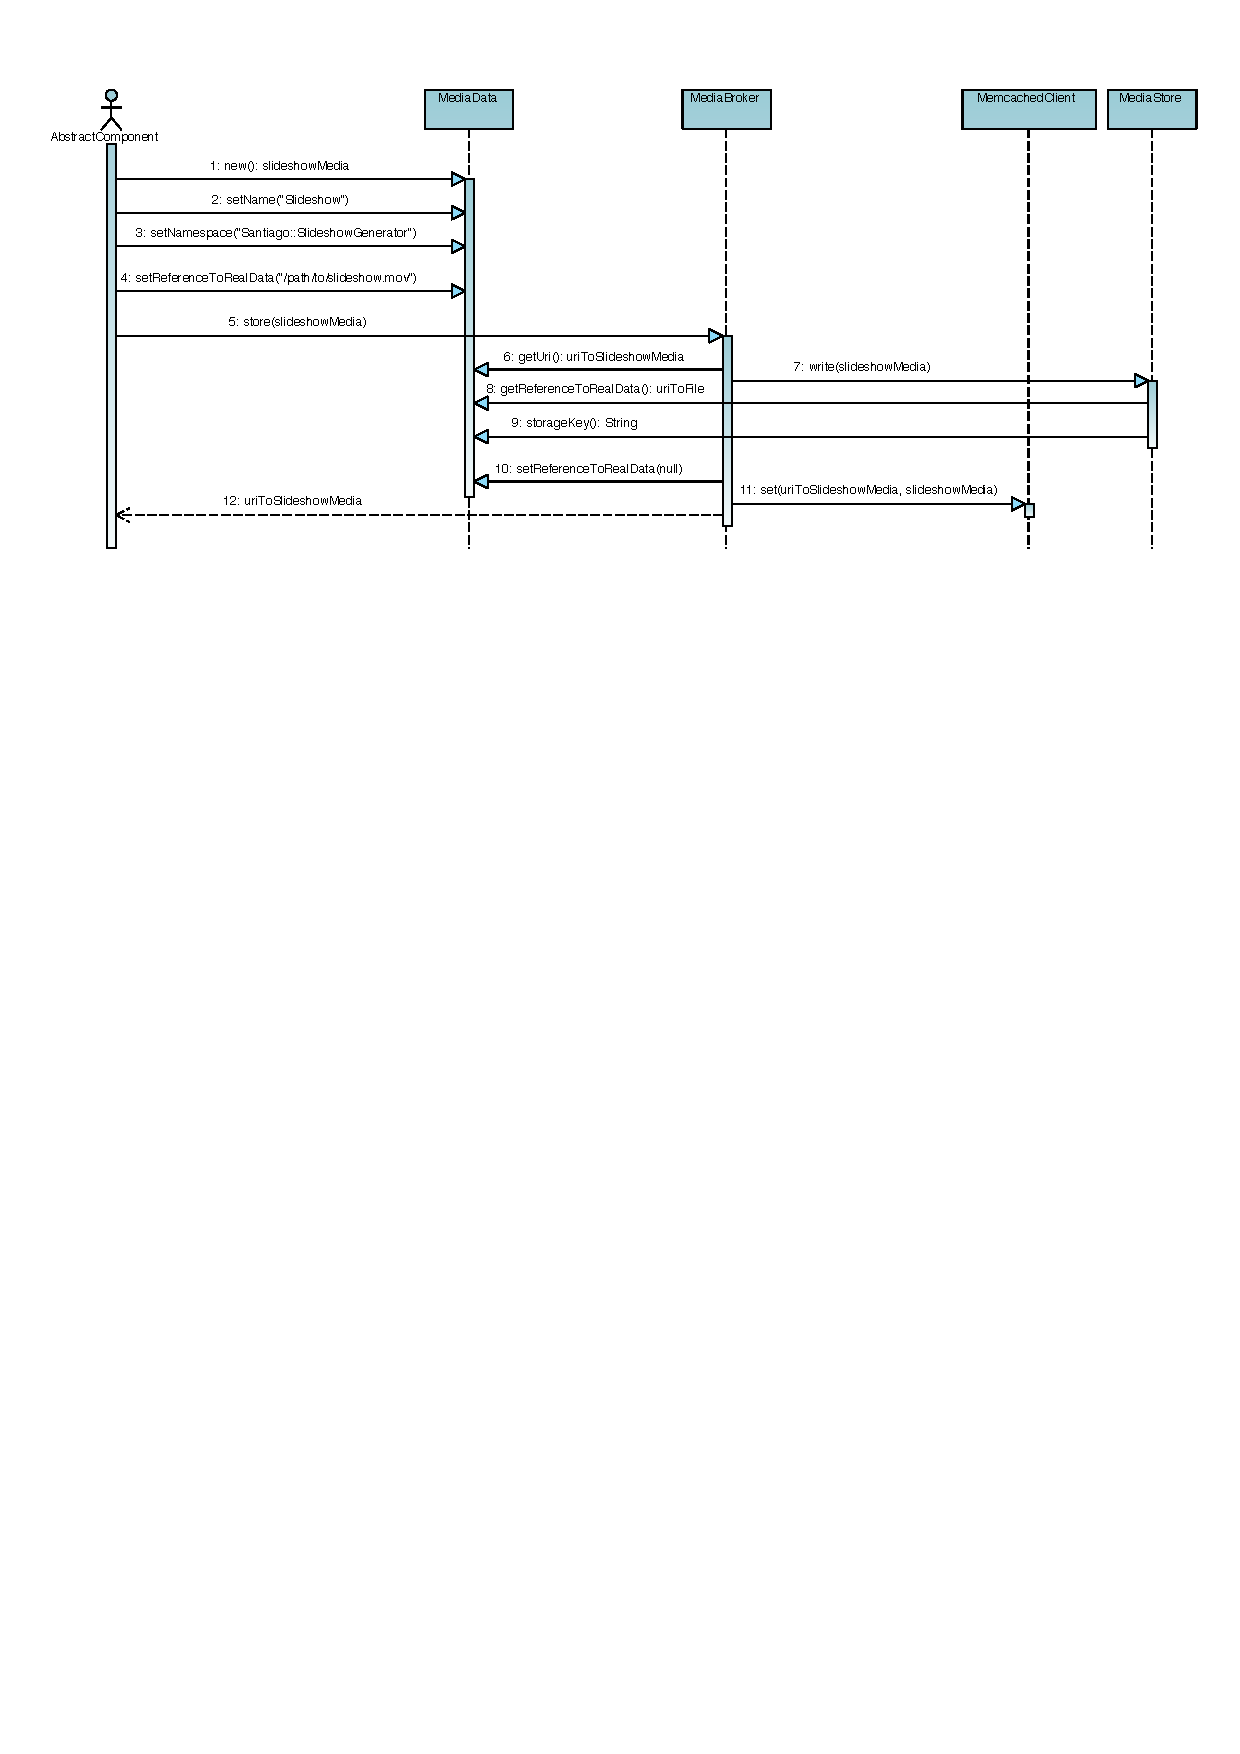
\includegraphics[width=\textwidth]{images/Handling_of_Media_Objects_write.pdf}
    \caption{Sequenzdiagramm über das Speichern von Medienobjekten}
    \label{fig:speichern_von_medienobjekten}
  \end{figure}
  
  Das Laden eines Medienobjekts wird durch die \verb!retrieve()!-Methode umgesetzt. Es wird dazu die URI eines Medienobjekts übergeben, anhand derer das entsprechende Objekt aus der implementierten Speicherlösung geholt wird. Um später über dieses Medienobjekt die eigentlichen Mediendaten über die die \verb!getPlayableData()!-Methode abrufen zu können, wird dem Medienobjekt noch die Referenz auf die \verb!MediaStore!-Instanz des Medienbrokers übergeben. Die Implementierung dieser Methode in der \verb!MemcachedMediaBroker!-Implementierung ist in Listing \ref{lst:retrieve_method_in_memcached_media_broker} zu sehen.

  \lstinputlisting[caption=Implementierung der \texttt{retrieve()}-Methode im  \texttt{MemcachedMediaBroker},label=lst:retrieve_method_in_memcached_media_broker,language=Java,firstline=62,lastline=66]{../code/COSIMA/src/main/java/de/fhkoeln/cosima/media/mediabroker/MemcachedMediaBroker.java}

  Das Sequenzdiagramm aus Abbildung \ref{fig:lesen_von_medienobjekten} verdeutlicht noch einmal die notwendigen Schritte, die beim lesen eines Medienobjekts notwendig sind.

  \begin{figure}[!ht]
    \centering
      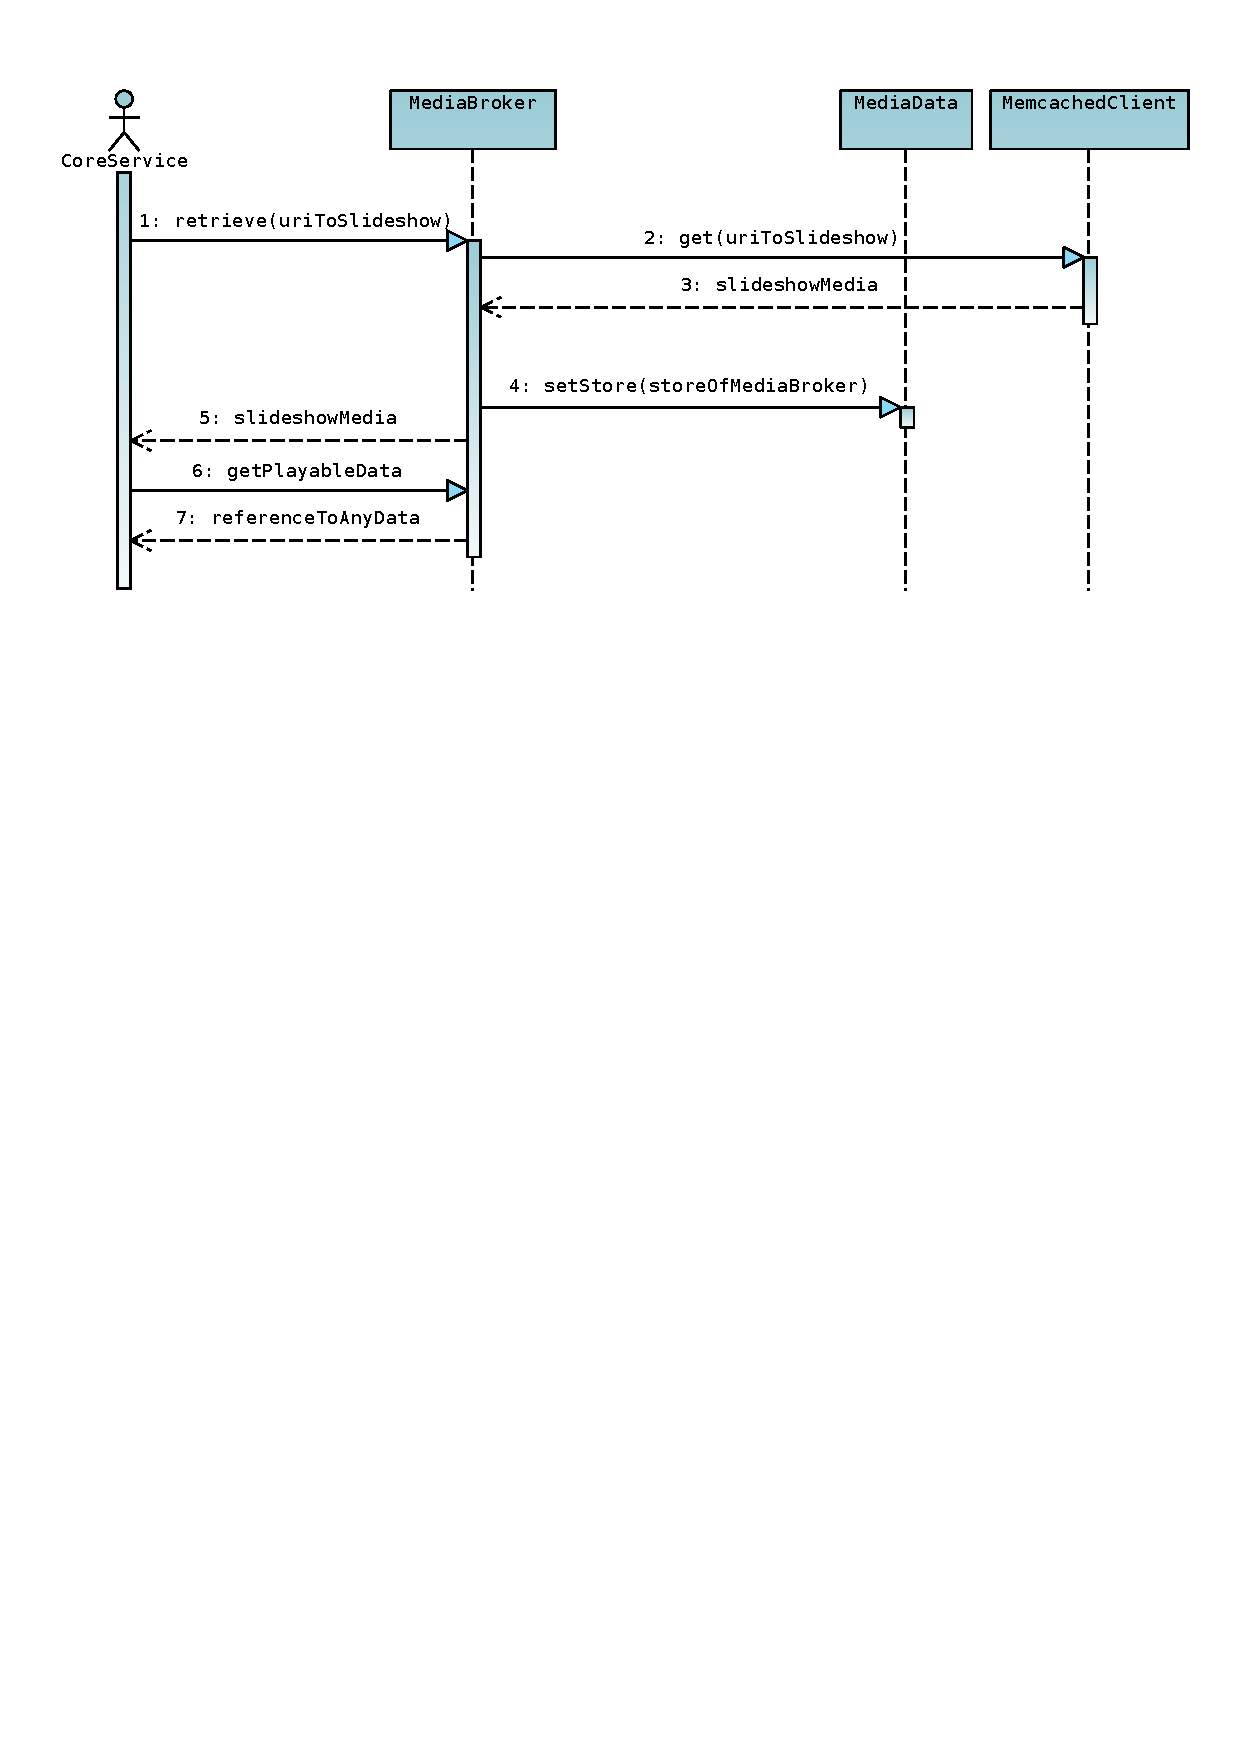
\includegraphics[width=\textwidth]{images/Handling_of_Media_Objects_read.pdf}
    \caption{Sequenzdiagramm über das Lesen von Medienobjekten}
    \label{fig:lesen_von_medienobjekten}
  \end{figure}

% subsubsection speichern_und_laden_von_medienobjekten (end)

  Stellvertretend für die anderen medienverarbeitenden Komponenten der Santiago-Anwendung ist in Listing \ref{lst:music_o_mat_with_media_object} die Implementierung der \verb!MusicOMat!-Klasse zur Integration des Medienobjekts dargestellt.

  \lstinputlisting[caption=Die \texttt{MusicOMat}-Klasse unter Verwendung des Medienobjekts,label=lst:music_o_mat_with_media_object,language=Java,firstline=26,lastline=42,morekeywords={[3]MediaComponent,getBroker,Media}]{../code/Santiago/src/main/java/de/fhkoeln/santiago/codesamples/MusicOMatWithMediaObject.java}
  
  Nachdem sowohl der explizite Kontrollfluss als auch der Datenfluss etabliert worden sind, bleibt als letzter Schritt nur noch die Umsetzung der einzelnen Komponenten als Dienste und ihre Verwendung in einer verteilten Umgebung. Dies wird im nächsten Abschnitt vorgestellt.
  
% subsection explizite_umsetzung_des_datenfluss (end)

\subsection{Extraktion der Komponenten als Dienste} % (fold)
\label{sub:extraktion_der_komponenten_als_dienste}

  Der letzte Schritt in der Umsetzung der Architektur war es, die medienverarbeitenden Komponenten so zu realisieren, dass sie auf unterschiedlichen Plattformen zum Einsatz kommen können. Im Rahmen dieser Arbeit wurde dieses Ziel durch die Realisierung der Komponenten als Web Services unter Verwendung von SOAP\abk{SOAP}{Simple Object Access Protocol} als Übertragungsprotokoll erreicht. Für die konkrete Implementierung der Web Service Kommunikation und SOAP wurde auf die \emph{Axis2 Web Service Engine}\footnote{\url{http://ws.apache.org/axis2/}} der Apache Group zurück gegriffen. Axis2 ist eine sehr mächtige Engine zum Betrieb von Web Services und wird in vielen Projekten eingesetzt. Da die Einbindung von Axis2 aber sehr transparent geschehen ist, kann leicht eine andere Lösung verwendet werden, wie etwa JAX-WS\footnote{\url{https://jax-ws.dev.java.net/}} oder Apache CXF\footnote{\url{http://cxf.apache.org/}}. Eine andere Alternative, die zur Auswahl stand war die Umsetzung einer REST\abk{REST}{Representational State Transfer}-Architektur. Da in einer REST-Architektur aber bestimmte Konventionen gelten\footnote{Wie etwa die Übertragung der HTTP\abk{HTTP}{Hypertext Transfer Protocol}-Verben (\lstinline[basicstyle=\ttfamily\footnotesize]{post}, \lstinline[basicstyle=\ttfamily\footnotesize]{get}, \lstinline[basicstyle=\ttfamily\footnotesize]{put}, \lstinline[basicstyle=\ttfamily\footnotesize]{delete}) auf die entsprechenden CRUD\abk{CRUD}{Create, Read, Update, Delete}-Operationen.} was nach \citep{service_oriented_computing} jedoch nicht eine Eigenschaft eines Dienstes sein sollte, weil sie eine lose Kopplung erschwert, wurde sich gegen diese Alternative entschieden.
  
\subsubsection{Definition einer Dienstschnittstelle} % (fold)
\label{ssub:definition_einer_dienstschnittstelle}

  Der erste Schritt bei der Umsetzung der Komponenten als Dienste war die Etablierung einer Schnittstelle, die die wesentlichen Methoden eines Dienstes definiert. Bei genauerer Betrachtung lässt sich schnell feststellen, dass nur die Methoden \verb!execute()! und \verb!setInput()! der \verb!AbstractComponent!-Klasse auch für die Veröffentlichung als Dienst von Relevanz sind. Das so entstandene \verb!CoreService!-Interface ist in Listing \ref{lst:core_service_interface} dargestellt.

  \lstinputlisting[caption=Das \texttt{CoreService}-Interface von COSIMA,label=lst:core_service_interface,language=Java,firstline=12]{../code/COSIMA/src/main/java/de/fhkoeln/cosima/services/CoreService.java}
  
  Die beiden Konstanten \verb!SERVICE_SET_INPUT_OPERATION! und \verb!SERVICE_EXECUTE_OPERATION! dienen dazu, die Informationen über die tatsächlichen Methoden an einer zentralen Stelle im \verb!CoreService!-Interface vorzuhalten. Zusätzlich wurden in dem Interface die beiden Methoden \verb!getUri()! und \verb!getDescription()! definiert, die zur Lokalisierung eines Dienstes über die Service Registry von Bedeutung sind. Diese wird im nächste Abschnitt genauer vorgestellt.

% subsubsection definition_einer_dienstschnittstelle (end)
  
\subsubsection{Umsetzung der Service Registry} % (fold)
\label{ssub:umsetzung_der_service_registry}

  Nachdem die einzelnen Komponenten über eine Schnittstelle verfügten, die sie als Dienste identifiziert, war der nächste Schritt, die Umsetzung der in Abschnitt \ref{ssub:definitionen_dienst} definierten Eigenschaft nach \emph{location transparency} \citep{service_oriented_computing}. Der Ort eines Dienstes soll demnach an einer zentralen Stelle hinterlegt werden. Im Prototypen wird diese Funktionalität durch die eine Implementierung des \verb!ServiceRegistry!-Interface aus Listing \ref{lst:service_registry_interface} bereitgestellt. Alternativ dazu hätte auch auf die bereits erwähnten Technologien UDDI oder ebXML zurückgegriffen werden können. Wie bereits in Bezug auf den Verzicht von BPEL ist auch hier anzuführen, dass eine Verwendung von UDDI oder ebXML nicht zielführend gewesen wäre. Daher wurde für den Prototypen eine \verb!ServiceRegistry!-Implementierung ebenfalls auf \verb!memcached!-Basis gewählt, ähnlich der des Medienbrokers. Dadurch ist die Service Registry selbst nicht als echter Dienst wie bei \citep{service_oriented_computing} gefordert implementiert, eignet sich aber dennoch für den Einsatz in einer verteilten Umgebung. Die Verwendung von JNDI\abk{JNDI}{Java Naming and Directory Interface} war dem gegenüber keine Option, da sie an die Java Plattform gebunden ist, was mit der Forderung nach Plattformunabhängigkeit \citep{service_oriented_computing} im Konflikt steht.

  \lstinputlisting[caption=Das \texttt{ServiceRegistry}-Interface von COSIMA,label=lst:service_registry_interface,language=Java,firstline=12]{../code/COSIMA/src/main/java/de/fhkoeln/cosima/services/registry/ServiceRegistry.java}

  Durch die Einführung einer Service Registry ist es auch nicht länger notwendig die tatsäch\-liche URI zu einer Komponente in der deklarativen Ablaufbeschreibung zu definieren. Es muss aber eine Beschreibung angegebenen werden anhand sich ein passender Dienst in der Registry finden lässt.
  
% subsubsection umsetzung_der_service_registry (end)

\subsubsection{Web Service-fähige Workflow Engine} % (fold)
\label{ssub:web_service_faehige_workflow_engine}

  Bevor sich der Inbetriebsetzung der Komponenten als Dienste zugewandt werden kann, muss zuvor eine \verb!WorkflowEngine!-Implementierung umgesetzt werden, die in der Lage ist diese Komponenten via SOAP aufzurufen und nicht länger über die Reflection API. Zu diesem Zwecke ist die \verb!RemoteWorkflowEngine! implementiert worden, deren vollständiges Listing \ref{lst:remote_workflow_engine} im Anhang zu finden ist. Die hier wesentliche Funktionalität für das Aufrufen eines Web Services findet sich in Listing \ref{lst:invoke_service} wieder.
  
  \lstinputlisting[caption=Aufruf eines Web Service aus der \texttt{RemoteWorkflowEngine} heraus,label=lst:invoke_service,language=Java,linerange={161-171,173-175,185-205}]{../code/COSIMA/src/main/java/de/fhkoeln/cosima/workflow/RemoteWorkflowEngine.java}
  
  Im Zuge dessen wurde auch das \verb!ProcessStore!-Interface aus Listing \ref{lst:process_store_interface} eingeführt, dass die Speicherung des Workflow-Fortschritts kapselt. Über dieses Interface lassen in späteren Versionen leicht verteilte Speicherstrategien verwenden, die somit auch eine verteilte Implementierung der \verb!WorkflowEngine! ermöglicht.
  
  \lstinputlisting[caption=Das \texttt{ProcessStore}-Interface,label=lst:process_store_interface,language=Java,firstline=12]{../code/COSIMA/src/main/java/de/fhkoeln/cosima/workflow/storage/ProcessStore.java}
  
  Zum Abschluss ist der Prozess der Ausführung in Abbildung \ref{fig:images_WorkflowEngine_Flowchart} noch einmal schematisch dargestellt.
  
  \begin{figure}[!ht]
    \centering
      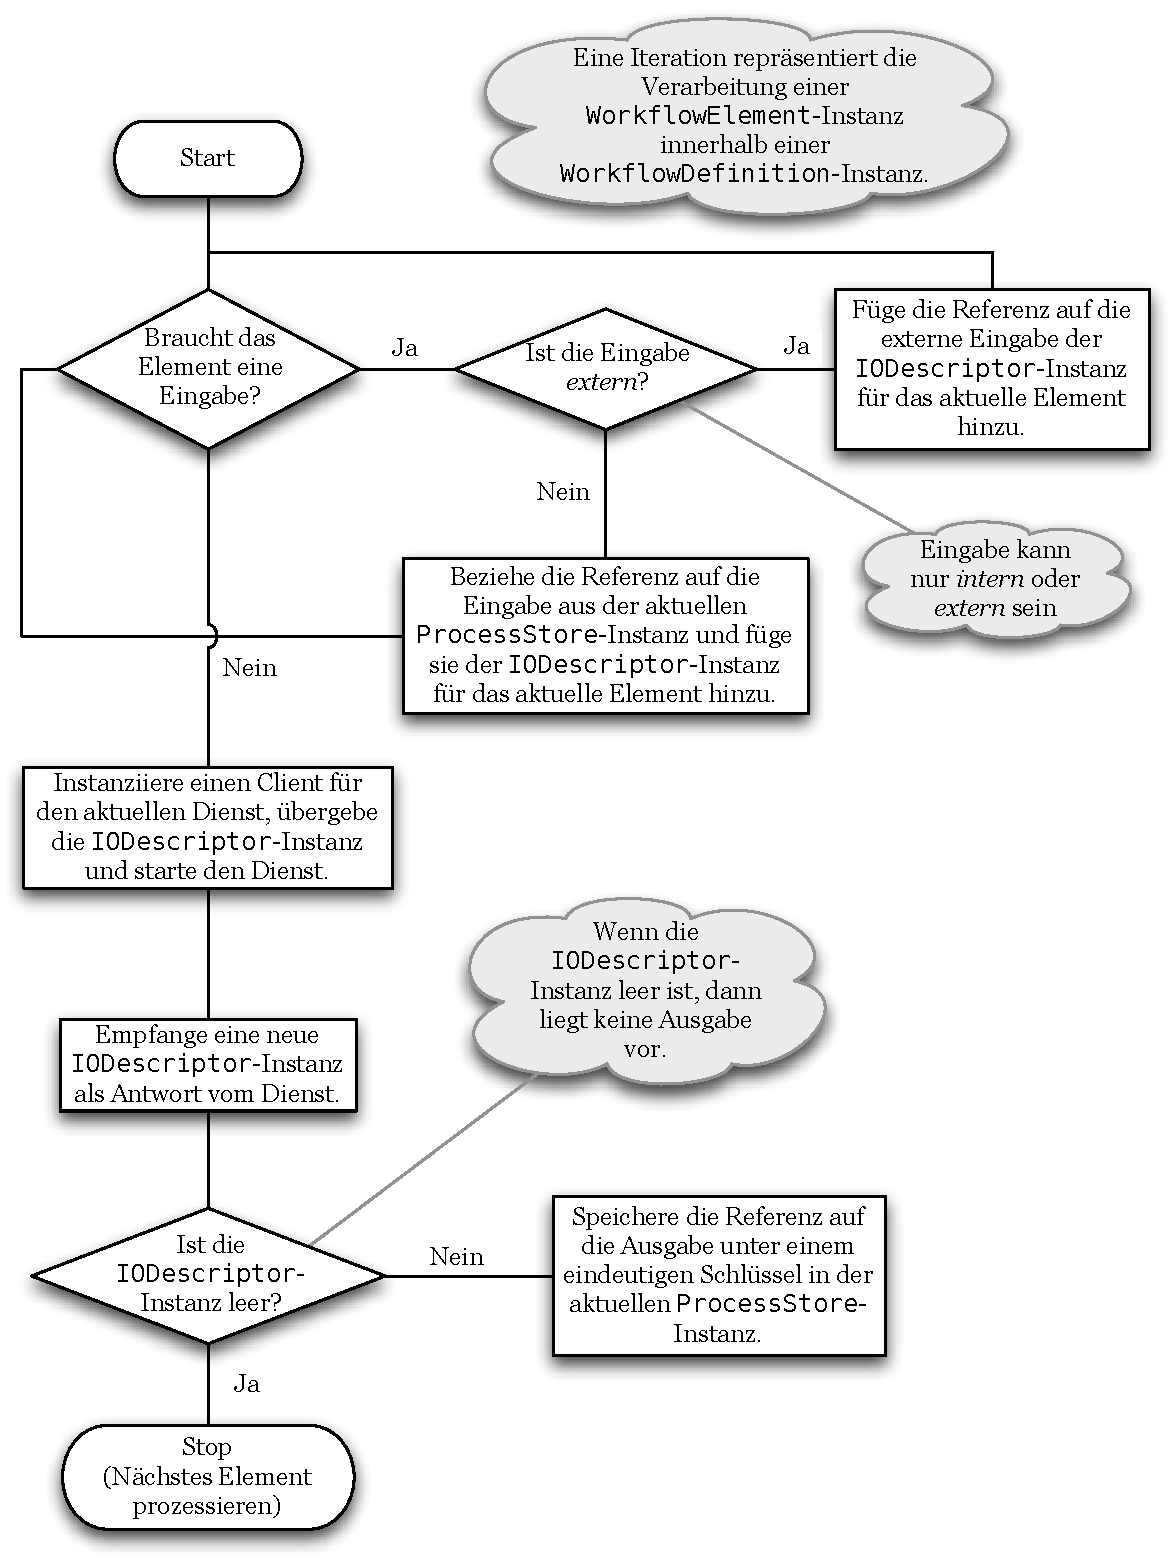
\includegraphics[width=.7\textwidth]{images/WorkflowEngine_Flowchart.pdf}
    \caption{Abalaufdiagramm für die \texttt{RemoteWorkflowEngine}}
    \label{fig:images_WorkflowEngine_Flowchart}
  \end{figure}

% subsubsection web_service_faehige_workflow_engine (end)

\subsubsection{Anpassung der Komponenten} % (fold)
\label{ssub:anpassung_der_komponenten}

  Als letzter Schritt musste die \verb!AbstractComponent!-Klasse angepasst werden ebenso wie die einzelnen medienverarbeitenden Komponenten. Die \verb!AbstractComponent!-Klasse implementiert nun das \verb!CoreService!-Interface und registriert bei Instanziierung sich selbst bei der Service Registry. Das vollständige Listing \ref{lst:abstract_component_final} der finalen Version der \verb!AbstractComponent!-Klasse mit allen Anpassungen findet sich im Anhang.
  
  Die Implementierung des \verb!MusicOMatService! in Listing \ref{lst:music_o_mat_service} steht exemplarisch für die Umsetzung der anderen Komponenten als Dienste. Zu beachten ist, dass die Klasse selbst die Adresse und Beschreibung des Dienstes definiert. Diese Informationen werden über den \verb!super()!-Konstruktor in der Service Registry veröffentlicht, so dass sich später der Dienst darüber wieder finden lässt.

  \lstinputlisting[caption=\texttt{MusicOMatService}-Klasse in der finalen Version,label=lst:music_o_mat_service,language=Java,linerange={12-13,26-61,86-87}]{../code/Santiago/src/main/java/de/fhkoeln/santiago/services/MusicOMatService.java}

  Die Dienste werden anschließen auf einem Tomcat Servlet Container\footnote{\url{http://tomcat.apache.org/}} über ein dort befindliches Axis2-Servlet verfügbar gemacht. Die Instanziierung der Dienste und die Auflösung der notwendigen Abhängigkeiten werden im Prototypen durch das Spring Framework\footnote{\url{http://www.springsource.org/}} auf Basis des \emph{Dependency Injection}-Pattern realisiert \citep[S. 130]{johnson2004eoo} und \citep{fowler04di}. In Listing \ref{lst:application_context} ist dabei die entsprechende Spring Konfigurationsdatei zu sehen.

  \lstinputlisting[caption=\texttt{applicationContext.xml}-zur Definition der Abhängigkeiten,label=lst:application_context,language=XML,linerange={1-2,18-57}]{../code/Santiago/src/main/resources/applicationContext.xml}
  
% subsubsection anpassung_an_den_komponenten (end)

\subsubsection{Die fertige Anwendung} % (fold)
\label{ssub:die_fertige_anwendung}

  Nachdem nun auch die Komponenten als Dienste realisiert sind und über Web Services auf einem Server zur Ausführung bereitstehen, muss nur noch das Santiago-Hauptprogramm wie in Listing \ref{lst:santiago_final_app} angepasst werden, so dass die \verb!RemoteWorkflowEngine! verwendet wird. Das Ergebnis ist die Erstellung und Wiedergabe einer Diashow mit Hintergrundmusik in einer verteilten und dienstorientierten Umgebung unter Verwendung des COSIMA-Projekts, wie es im vorherigen Kapitel beschrieben wurde.

  \lstinputlisting[caption=Die finale Version der Santiago Anwendung,label=lst:santiago_final_app,language=Java]{../code/Santiago/src/main/java/de/fhkoeln/santiago/SantiagoApp.java}
  
% subsubsection die_fertige_anwendung (end)

% subsection extraktion_der_komponenten_als_dienste (end)
  
% section realisierung_der_architektur (end)

\section{Realisierung des Szenario (Nerstrand)} % (fold)
\label{sec:realisierung_des_szenario}

  Nachdem im vorherigen Abschnitt erfolgreich die COSIMA-Architektur realisiert wurde kann nun das eigentliche Szenario aus Abschnitt \ref{sub:das_anwendungsszenario} auf Basis dieser Architektur implementiert werden. Zur Entwicklung und zur besseren Kommunikation hat diese Anwendung den Codenamen \emph{Nerstrand} erhalten. Bevor die wesentlichen Komponenten, die es umzusetzen galt, vorgestellt werden, soll zunächst das eigentliche Anwendungsprogramm aus Listing \ref{lst:nerstrand_app} diskutiert werden.
  
  \lstinputlisting[caption=Die Nerstrand Anwendung als Umsetzung des Szenario,label=lst:nerstrand_app,language=Java,linerange={1-2,13-35}]{../code/nerstrand/src/main/java/de/fhkoeln/nerstrand/NerstrandApp.java}
  
  Wie sich leicht erkennen lässt bestehen keinerlei Unterschiede zum Anwendungsprogramm von Santiago aus Listing \ref{lst:santiago_final_app}. Auch sonst ist Nerstrand ähnlich umgesetzt worden wie Santiago: Die Dienste werden auch hier über einen Tomcat Servlet Container verfügbar gemacht und die Auflösung der Abhängigkeiten geschieht ebenso über Dependency Injection und das Spring Framework. Und genau das was das erwartete Ergebnis, denn eine Anwendung, die sich des COSIMA-Projekts bedient, wird über eine Ablaufbeschreibung definiert sowie über die Implementierung spezifischer Dienste realisiert. Daher sollten auch nur diese beiden Elemente angepasst werden müssen. Die Ablaufbeschreibung in Listing \ref{lst:nerstrand_workflow_definition} ist für die Nerstrand Anwendung ist sogar noch einfacher geworden, als die der Santiago Anwendung, da nur ein Producer- sowie ein Consumer-Dienst benötigt werden.

  \lstinputlisting[caption=Die Ablaufbeschreibung für die Nerstrand Anwendung,label=lst:nerstrand_workflow_definition,language=YAML]{../code/nerstrand/src/main/resources/workflow_definition.yml}
  
  Selbst der Consumer-Dienst unterscheidet sich nur marginal von dem Consumer-Dienst in Santiago. Daher soll an dieser Stelle vor allem der Producer-Dienst vorgestellt werden, der das Webcam Signal abgreift und als Stream bereitstellt. Die Implementierung der wesentlichen Funktionalitäten dieses Dienst lässt sich Listing \ref{lst:webcam_streaming_service} entnehmen.
  
  \lstinputlisting[caption=Der \texttt{WebcamStreamingService} der Nerstrand Anwendung,label=lst:webcam_streaming_service,language=Java,linerange={12-13,26-33,39-59,92-93},morekeywords={[3]thread,while,VLCStreamingOperation,streamingOp}]{../code/nerstrand/src/main/java/de/fhkoeln/nerstrand/services/WebcamStreamingService.java}
  
  Der Eigentliche Streamingprozess ist dabei in der \verb!VLCStreamingOperation!-Klasse gekapselt worden. Dies geschah aus zwei Gründen: Zum einen ist die Funktionalität dadurch in Isolation leichter zu testen, zum anderen, und das ist der entscheidende Grund, lässt sich die Operation in einem Thread starten. Dies ist notwendig, da die Operation kein definiertes Ende hat, wie etwa die Operationen in der Santiago Anwendung. Als Lösung wird der Streamingvorgang über die \verb!thread()!-Methode aus Zeile 49 in einem Thread ausgeführt und die \verb!execute()!-Methode kann dadurch regulär beendet werden. Das bedeutet, dass überhaupt erst das \verb!stream!-Medienobjekt im Medienbroker gespeichert werden kann und die \verb!output!-Instanz mit den notwendigen Informationen an den Dienstnutzer zurückgegeben werden wird. Wäre das nicht der Fall würde der gesamte Workflow zum erliegen kommen, da die Eingabe für den folgenden Dienst nicht gefunden werden kann.
  
  Eine andere Besonderheit bestand bei der Implementierung der \verb!VLCStreamingOperation!. Da der verwendete \verb!MediaStore! nur in der Lage ist Dateien abzulegen, war es notwendig die Informationen als Datei zu repräsentieren. Als Lösung dieses Problems werden die Informationen über den Stream in einer SDP\abk{SDP}{Session Description Protocol}-Datei abgelegt. SDP steht für \emph{Session Description Protocol} und dient dazu Informationen wie die Kodierung der Daten, Transportprotokoll, Ziel- und Ursprungsadresse des Streams sowie den verwendeten Port in einer standardisierten Form zu repräsentieren\footnote{\url{http://tools.ietf.org/html/rfc4566}}. Diese Datei kann dann von der \verb!MediaStore!-Instanz gespeichert und von dem Consumer-Dienst später dazu verwendet werden den eigentlichen Stream wiederzugeben.

  Mehr als das hier beschriebene war nicht notwendig, um das Anwendungsszenario prototypisch zu implementieren. Die wenigen Schritte sind auf den ersten Blick bereits ein gutes Zeichen dafür, dass die Architektur geeignet ist Multimediaanwendungen zu realisieren. Eine genauere Betrachtung und vor allem eine Validierung der Implementierung und deren Ergebnisse erfolgt im folgenden Kapitel.

% section realisierung_des_szenario (end)

% chapter prototypische_realisierung (end)